\section{Analyse}

In diesem Kapitel wird die bestehende Situation im Budget-Controlling analysiert und die Anforderungen an die zu entwickelnde Middleware definiert. Die Analyse folgt nach \cite{sommerville2015} einem strukturierten Vorgehen: Zunächst wird der Ist-Zustand erfasst, anschließend werden funktionale und nicht-funktionale Anforderungen abgeleitet.

\subsection{Ist-Analyse}

\subsubsection{Excel-basierter Workflow}

Der aktuelle Workflow im Budget-Controlling basiert auf einer zentralen Excel-Datei (\texttt{Budgetcontrolling.xlsx}), die über SharePoint mit allen Beteiligten geteilt wird. Die Datei aggregiert Daten aus mehreren Quellen mittels Power Query: User Stories und ihre Aufwände werden automatisch aus SAP \gls{calm} abgerufen, Zeitbuchungen stammen aus einem SAP-Listenexport (CADO), und die Budget-Planung pro \gls{psp}-Element wird manuell gepflegt. Der Projektleiter öffnet die Datei, aktualisiert die Power-Query-Verbindungen und liest die daraus berechneten Kennzahlen ab. Manuelle \gls{psp}-Zuordnungen, die nicht in \gls{calm} hinterlegt sind, werden direkt in der Datei eingetragen. Tabelle~\ref{tab:excel-sheets} zeigt die einzelnen Sheets und ihre Datenquellen.

\begin{table}[H]
\centering
\caption{Sheets in Budgetcontrolling.xlsx}
\label{tab:excel-sheets}
\begin{tabularx}{\textwidth}{l>{\raggedright\arraybackslash}Xl}
\toprule
\textbf{Sheet} & \textbf{Zweck} & \textbf{Quelle} \\
\midrule
qry\_CALM\_Data & User Stories mit \gls{psp}-Zuordnung & Power Query \\
CADO & Zeitbuchungen (Ist-Stunden) & SAP-Export \\
PSP-Elemente & Budget pro \gls{psp} & Manuell \\
1. PSP-Zuordnung & Manuelle Zuordnungen & Manuell \\
2. PSP-Zuordnung & Fallback: Team $\rightarrow$ Timebox $\rightarrow$ \gls{psp} & Manuell \\
Reporting & Zusammenfassung pro Team & Berechnet \\
\bottomrule
\end{tabularx}
\end{table}

\subsubsection{Budget-Metriken}

Die folgenden Metriken werden für das Budget-Controlling verwendet. Diese Kennzahlen entsprechen den im Projektmanagement etablierten Earned Value Management (EVM) Metriken \citep{kerzner2017, pmi2021}:

\begin{table}[H]
\centering
\caption{Budget-Metriken und ihre Berechnung}
\label{tab:metriken}
\begin{tabularx}{\textwidth}{l>{\raggedright\arraybackslash}Xl}
\toprule
\textbf{Metrik} & \textbf{Beschreibung} & \textbf{Berechnung} \\
\midrule
Budget & Geplantes Budget & Summe aus PSP-Elemente \\
Actual & Bereits geleistete Arbeit & CADO Stunden / 8 \\
\gls{etc} & Noch zu leistende Arbeit & qry\_CALM\_Data (mit \gls{psp}) \\
\gls{eac} & Geschätzte Gesamtkosten & Actual + \gls{etc} \\
\bottomrule
\end{tabularx}
\end{table}

Zur Veranschaulichung ein Beispiel: Für ein Team mit einem geplanten Budget von 120~PT wurden bisher 55,53~PT tatsächlich geleistet (Actual), die aus den CADO-Zeitbuchungen berechnet werden (444,24 Stunden / 8). Der verbleibende Restaufwand (ETC) beträgt laut den User Stories mit \gls{psp}-Zuordnung 63,88~PT. Daraus ergibt sich eine Gesamtprognose (EAC) von 119,41~PT (55,53 + 63,88), die in diesem Fall knapp unter dem Budget liegt.

\subsubsection{Problemanalyse}

Die Analyse des bestehenden Workflows offenbart vier zentrale Probleme.

Das erste Problem betrifft die \textbf{fehlende Echtzeitfähigkeit}. Die Power-Query-Verbindungen in Excel werden nur bei manuellem Refresh aktualisiert. Zwischen zwei Aktualisierungen können Stunden oder Tage vergehen, in denen Entscheidungen auf veralteten Daten basieren. Insbesondere bei der ETC-Berechnung, die sich auf die Restaufwände der User Stories stützt, führt dies zu ungenauen Prognosen.

Das zweite Problem ist die \textbf{fehlende Programmierschnittstelle}. Die Budget-Daten sind ausschließlich innerhalb der Excel-Datei verfügbar. Es existiert keine \gls{api}, über die ein Frontend, ein Dashboard oder andere Systeme programmatisch auf die Kennzahlen zugreifen könnten. Jede Auswertung erfordert das manuelle Öffnen und Lesen der Datei.

Das dritte Problem betrifft die \textbf{fehlende Konsistenzprüfung}. \gls{psp}-Zuordnungen werden manuell in Excel eingetragen, ohne dass eine automatische Validierung stattfindet. So können User Stories einem \gls{psp}-Element zugeordnet werden, dessen Team nicht mit dem Team der User Story übereinstimmt (\textit{Team-Mismatch}), was zu fehlerhaften Budget-Aggregationen führt.

Das vierte Problem ist die \textbf{mangelnde Nachvollziehbarkeit}. Änderungen an den \gls{psp}-Zuordnungen werden nicht protokolliert. Es ist nicht ersichtlich, wer wann welche Zuordnung erstellt oder geändert hat. Dies erschwert die Fehlersuche und die Kontrolle der Datenqualität.

\subsection{Soll-Konzept}

Die Middleware soll die beschriebenen Probleme lösen und gleichzeitig einen einfachen Übergang zu einer service-orientierten Architektur ermöglichen. Middleware bezeichnet dabei Software, die als Vermittlungsschicht zwischen verteilten Anwendungen fungiert und deren Kommunikation vereinfacht \citep{bernstein1996, tanenbaum2017}.

Das Konzept folgt dem Prinzip der \enquote{Strangler Fig Application} \citep{newman2021}: Anstatt das bestehende Excel-basierte System vollständig abzulösen, wird zunächst eine Middleware eingeführt, die die Excel-Daten über eine standardisierte \gls{api} bereitstellt. Das Frontend kommuniziert ausschließlich mit der Middleware und hat keine Kenntnis über die zugrundeliegende Datenquelle. In einem späteren Schritt kann die Excel-Datenquelle durch OData-Services von SAP \gls{calm} ersetzt werden, ohne dass das Frontend angepasst werden muss. Die Middleware übernimmt somit die Rolle des \enquote{Stranglers}, der das alte System schrittweise durch eine neue Architektur ersetzt.

\begin{figure}[H]
\centering
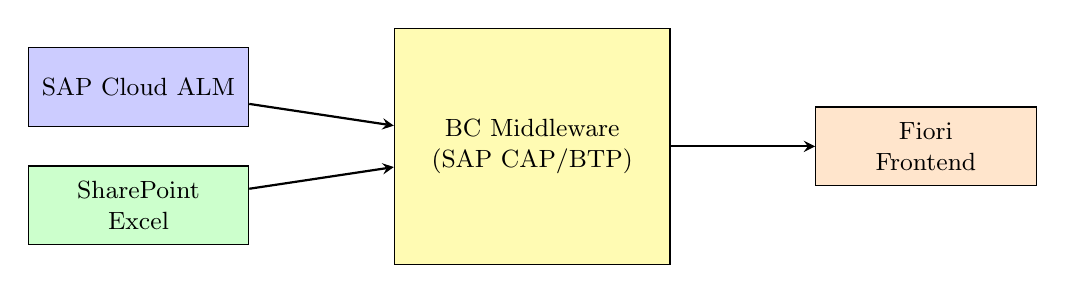
\begin{tikzpicture}[
    box/.style={rectangle, draw, minimum width=2.8cm, minimum height=1cm, align=center, font=\small},
    arrow/.style={->, >=stealth, thick}
]
    % Datenquellen links
    \node[box, fill=blue!20] (calm) at (0,1.5) {SAP Cloud ALM};
    \node[box, fill=green!20] (sharepoint) at (0,0) {SharePoint\\Excel};

    % Middleware Mitte
    \node[box, fill=yellow!30, minimum width=3.5cm, minimum height=3cm] (middleware) at (5,0.75) {BC Middleware\\(SAP CAP/BTP)};

    % Frontend rechts
    \node[box, fill=orange!20] (frontend) at (10,0.75) {Fiori\\Frontend};

    % Pfeile
    \draw[arrow] (calm) -- (middleware);
    \draw[arrow] (sharepoint) -- (middleware);
    \draw[arrow] (middleware) -- (frontend);
\end{tikzpicture}
\caption{Soll-Architektur der BC Middleware}
\label{fig:soll-architektur}
\end{figure}

Abbildung~\ref{fig:soll-architektur} zeigt die resultierende Zielarchitektur. Die Middleware nimmt Daten von beiden möglichen Backends entgegen und stellt sie dem Frontend über eine einheitliche \gls{odata} v4-Schnittstelle zur Verfügung.

\subsection{Verwandte Arbeiten}

Die Problemstellung der vorliegenden Arbeit berührt mehrere Forschungsbereiche, die im Folgenden eingeordnet werden.

\subsubsection{Middleware und Integrationsarchitekturen}

Das Konzept der Middleware als Vermittlungsschicht zwischen heterogenen Systemen ist seit den 1990er Jahren etabliert \citep{bernstein1996}. \cite{emmerich2000} identifizierte Middleware als zentrales Element für die Integration verteilter Systeme und prognostizierte deren wachsende Bedeutung. Die Enterprise Integration Patterns von \cite{hohpe2003} bieten einen umfassenden Katalog von Integrationsmustern, darunter das in dieser Arbeit verwendete Adapter-Pattern.

\subsubsection{Spreadsheet-basierte Systeme in Unternehmen}

Die Verbreitung und Risiken von Spreadsheet-Anwendungen in Unternehmen sind Gegenstand umfangreicher Forschung. \cite{panko2016} beschreiben Tabellenkalkulationen als \enquote{Dark Matter} der Unternehmens-IT -- allgegenwärtig, aber schwer zu kontrollieren. \cite{powell2009} dokumentieren in ihrer Metastudie, dass Spreadsheets häufig Fehler enthalten und dennoch für geschäftskritische Entscheidungen verwendet werden. Diese Erkenntnisse unterstreichen die Relevanz von Lösungen, die einen kontrollierten Übergang zu strukturierteren Systemen ermöglichen.

\subsubsection{Abgrenzung}

Im Unterschied zu bestehenden Arbeiten, die sich primär auf die Fehleranalyse von Spreadsheets oder allgemeine Integrationsarchitekturen konzentrieren, adressiert diese Arbeit die spezifische Fragestellung der Backend-Austauschbarkeit im SAP-Kontext. Der Fokus liegt auf der praktischen Umsetzung einer Architektur, die sowohl Excel-basierte als auch service-orientierte Backends unterstützt.

\subsection{Stakeholder-Analyse}

Für den erfolgreichen Entwurf der Middleware ist das Verständnis der beteiligten Stakeholder und ihrer Anforderungen essentiell \citep{sommerville2015}. Tabelle~\ref{tab:stakeholder} zeigt die identifizierten Stakeholder-Gruppen. Dabei sind teilweise gegenläufige Interessen erkennbar: Während Projektleiter und Controller vor allem an korrekten Daten und einfacher Bedienung interessiert sind, legen die Frontend-Entwickler Wert auf eine stabile, dokumentierte \gls{api}. Die IT-Architekten wiederum priorisieren die langfristige Austauschbarkeit des Backends. Die Middleware muss diese unterschiedlichen Perspektiven berücksichtigen und insbesondere sicherstellen, dass die \gls{api}-Stabilität nicht durch spätere Backend-Wechsel beeinträchtigt wird.

\begin{table}[H]
\centering
\caption{Stakeholder und ihre Interessen}
\label{tab:stakeholder}
\begin{tabularx}{\textwidth}{l>{\raggedright\arraybackslash}X>{\raggedright\arraybackslash}X}
\toprule
\textbf{Stakeholder} & \textbf{Rolle} & \textbf{Interesse} \\
\midrule
Projektleiter & Nutzt Budget-Reports für Entscheidungen & Aktuelle, korrekte Zahlen; einfache Bedienung \\
\midrule
Controller & Pflegt Budgetdaten und PSP-Zuordnungen & Effiziente Dateneingabe; Konsistenzprüfung \\
\midrule
Frontend-Entwickler & Entwickelt Fiori-Oberfläche & Stabile, dokumentierte API; OData-Konformität \\
\midrule
IT-Architekten & Plant zukünftige Integration & Austauschbarkeit; saubere Architektur \\
\midrule
SAP-Administratoren & Betreibt die Anwendung auf BTP & Einfaches Deployment; Monitoring \\
\bottomrule
\end{tabularx}
\end{table}

\subsection{Use Cases}

Die folgenden Use Cases beschreiben die wichtigsten Interaktionen mit der Middleware-API. Da die vorliegende Arbeit ausschließlich die OData-Schnittstelle bereitstellt und kein Frontend umfasst (siehe Abschnitt~\ref{sec:abgrenzung}), sind die Akteure jeweils API-Konsumenten -- etwa ein Fiori-Frontend oder ein REST-Client \citep{sommerville2015}.

\subsubsection{UC-01: Budget-Übersicht abrufen}

\begin{table}[H]
\centering
\begin{tabularx}{\textwidth}{l>{\raggedright\arraybackslash}X}
\toprule
\textbf{Akteur} & API-Konsument (z.\,B. Fiori-Frontend) \\
\midrule
\textbf{Vorbedingung} & Eine gültige Session-ID liegt vor (\texttt{x-session-id} Header) \\
\midrule
\textbf{Ablauf} &
1. Client sendet \texttt{GET /api/budget/BudgetOverview} mit \texttt{x-session-id} Header \\
& 2. Middleware validiert die Session und ermittelt das zugehörige Projekt \\
& 3. Middleware lädt die Excel-Datei des Projekts und berechnet die Budget-Metriken \\
& 4. Middleware gibt ein OData-konformes JSON-Array mit Budget, Actual, ETC und EAC pro Team zurück \\
\midrule
\textbf{Nachbedingung} & Client erhält die berechneten Budget-Metriken als OData-Response \\
\bottomrule
\end{tabularx}
\caption{Use Case: Budget-Übersicht abrufen}
\end{table}

\subsubsection{UC-02: PSP-Zuordnung erstellen}

\begin{table}[H]
\centering
\begin{tabularx}{\textwidth}{l>{\raggedright\arraybackslash}X}
\toprule
\textbf{Akteur} & API-Konsument (z.\,B. Fiori-Frontend) \\
\midrule
\textbf{Vorbedingung} & Gültige Session; User Story existiert ohne PSP-Zuordnung \\
\midrule
\textbf{Ablauf} &
1. Client sendet \texttt{POST /api/budget/createPSPAssignment} mit den Parametern \texttt{userStory}, \texttt{psp}, \texttt{teamUserStory} und \texttt{teamPSP} \\
& 2. Middleware prüft, ob die Zuordnung bereits existiert (bei Duplikat: \texttt{409 Conflict}) \\
& 3. Middleware schreibt die Zuordnung in das Sheet \enquote{1. PSP-Zuordnung} der Excel-Datei \\
& 4. Middleware gibt eine Bestätigung mit der erstellten Zuordnung zurück \\
\midrule
\textbf{Nachbedingung} & Die Zuordnung ist in der Excel-Datei persistiert; nachfolgende Abfragen berücksichtigen das neue PSP in der ETC-Berechnung \\
\midrule
\textbf{Alternativ} & Unterscheiden sich \texttt{teamUserStory} und \texttt{teamPSP}, enthält die Response eine Team-Mismatch-Warnung \\
\bottomrule
\end{tabularx}
\caption{Use Case: PSP-Zuordnung erstellen}
\end{table}

\subsubsection{UC-03: Session starten und Projekt wählen}

\begin{table}[H]
\centering
\begin{tabularx}{\textwidth}{l>{\raggedright\arraybackslash}X}
\toprule
\textbf{Akteur} & API-Konsument (z.\,B. Fiori-Frontend) \\
\midrule
\textbf{Vorbedingung} & Mindestens ein Projekt ist in \texttt{excel\_templates/} konfiguriert \\
\midrule
\textbf{Ablauf} &
1. Client sendet \texttt{GET /api/budget/getProjects()} und erhält eine Liste verfügbarer Projekte \\
& 2. Client sendet \texttt{POST /api/budget/startSession} mit dem gewählten Projektnamen \\
& 3. Middleware erstellt eine Session im Arbeitsspeicher und gibt eine Session-ID zurück \\
& 4. Client speichert die Session-ID und sendet sie bei allen folgenden Requests im \texttt{x-session-id} Header \\
\midrule
\textbf{Nachbedingung} & Alle nachfolgenden API-Aufrufe mit dieser Session-ID beziehen sich auf das gewählte Projekt \\
\bottomrule
\end{tabularx}
\caption{Use Case: Session starten und Projekt wählen}
\end{table}

\subsection{Anforderungsanalyse}

\subsubsection{Funktionale Anforderungen}

Die funktionalen Anforderungen leiten sich direkt aus den Use Cases und der Problemanalyse ab. Sie beschreiben, \textit{was} das System leisten muss. Die Budget-Metriken (FA-01, FA-02) adressieren die Kernfunktionalität der Middleware. Die \gls{psp}-Zuordnungen (FA-03, FA-07) lösen das Problem der fehlenden Konsistenzprüfung, indem sie eine kontrollierte Schnittstelle für Änderungen bereitstellen. Das Session-Management (FA-04) ermöglicht die gleichzeitige Unterstützung mehrerer Projekte. Tabelle~\ref{tab:fa} gibt einen Überblick.

\begin{table}[H]
\centering
\caption{Funktionale Anforderungen}
\label{tab:fa}
\begin{tabularx}{\textwidth}{l>{\raggedright\arraybackslash}X}
\toprule
\textbf{ID} & \textbf{Anforderung} \\
\midrule
FA-01 & Das System muss Budget-Metriken pro Team berechnen können \\
FA-02 & Das System muss Budget-Metriken pro \gls{psp} berechnen können \\
FA-03 & Das System muss \gls{crud}-Operationen für \gls{psp}-Zuordnungen unterstützen \\
FA-04 & Das System muss Session-basiertes Projekt-Management unterstützen \\
FA-05 & Das System muss Team-Mismatch-Warnungen generieren können \\
FA-06 & Das System muss Excel-Daten von SharePoint lesen können \\
FA-07 & Das System muss Änderungen zurück in Excel schreiben können \\
\bottomrule
\end{tabularx}
\end{table}

\subsubsection{Nicht-funktionale Anforderungen}

Die nicht-funktionalen Anforderungen definieren Qualitätsmerkmale des Systems. Die zentrale Anforderung NFA-01 (Backend-Austauschbarkeit) spiegelt die Forschungsfrage dieser Arbeit wider und beeinflusst maßgeblich die Architekturentscheidungen in Kapitel~4. Die OData-Kompatibilität (NFA-02) und Fiori-Eignung (NFA-04) werden durch den Einsatz von SAP \gls{cap} sichergestellt. Der Verzicht auf eine lokale Datenbank (NFA-05) folgt aus der Designentscheidung, Excel als \textit{Single Source of Truth} beizubehalten.

\begin{table}[H]
\centering
\caption{Nicht-funktionale Anforderungen}
\label{tab:nfa}
\begin{tabularx}{\textwidth}{l>{\raggedright\arraybackslash}X}
\toprule
\textbf{ID} & \textbf{Anforderung} \\
\midrule
NFA-01 & Die Backend-Implementierung muss austauschbar sein \\
NFA-02 & Die \gls{api} muss \gls{odata} v4-kompatibel sein \\
NFA-03 & Das System muss auf der SAP \gls{btp} deploybar sein \\
NFA-04 & Die \gls{api} muss für ein Fiori-Frontend geeignet sein \\
NFA-05 & Das System muss ohne lokale Datenbankinstanz funktionieren \\
\bottomrule
\end{tabularx}
\end{table}

\subsection{Priorisierung der Anforderungen}

Die Anforderungen werden nach der MoSCoW-Methode priorisiert \citep{sommerville2015}. Die Einstufung orientiert sich daran, ob die Middleware ohne die jeweilige Anforderung ihren Kernzweck erfüllen kann. Budget-Metriken (FA-01, FA-02) und der Datenzugriff auf Excel (FA-06) bilden zusammen mit der OData-Kompatibilität (NFA-02) die \textit{Must}-Kategorie, da ohne sie kein funktionsfähiges System entsteht. Die \textit{Should}-Anforderungen (CRUD, Session-Management, Austauschbarkeit) erweitern die Funktionalität erheblich, sind jedoch für einen ersten Prototyp nicht zwingend erforderlich. Die \textit{Could}-Anforderungen (Warnungen, Write-Back) stellen Zusatzfunktionen dar, die den Nutzen steigern, aber auch später ergänzt werden können.

\begin{table}[H]
\centering
\caption{Priorisierung der Anforderungen}
\label{tab:priorisierung}
\begin{tabularx}{\textwidth}{cl>{\raggedright\arraybackslash}X}
\toprule
\textbf{Prio} & \textbf{ID} & \textbf{Anforderung} \\
\midrule
\multirow{4}{*}{\textbf{Must}} & FA-01 & Budget-Metriken pro Team \\
& FA-02 & Budget-Metriken pro PSP \\
& FA-06 & Excel-Daten lesen \\
& NFA-02 & OData v4-kompatibel \\
\midrule
\multirow{3}{*}{\textbf{Should}} & FA-03 & CRUD für PSP-Zuordnungen \\
& FA-04 & Session-Management \\
& NFA-01 & Backend austauschbar \\
\midrule
\multirow{2}{*}{\textbf{Could}} & FA-05 & Team-Mismatch-Warnungen \\
& FA-07 & Excel Write-Back \\
\midrule
\textbf{Won't} & -- & Fiori-Frontend (andere Arbeit) \\
\bottomrule
\end{tabularx}
\end{table}

\subsection{Abgrenzung}
\label{sec:abgrenzung}

Mehrere Aspekte sind bewusst nicht Bestandteil dieser Arbeit. Das Fiori-Frontend wird von anderen Studierenden im Rahmen separater Arbeiten entwickelt; die vorliegende Arbeit stellt lediglich die API bereit. Die vollständige CALM-Integration wird nur konzeptionell beschrieben, aber nicht implementiert, was dennoch eine Bewertung der Austauschbarkeit ermöglicht. Die Benutzer-Authentifizierung wird durch die SAP BTP (XSUAA Service) bereitgestellt und ist somit nicht Teil der Middleware-Implementierung. Eine vollständige Audit-Trail-Funktionalität für die Historisierung von Änderungen ist ebenso wenig vorgesehen wie eine vollständige Mandantentrennung mit separaten Datenbeständen -- die Middleware unterstützt zwar mehrere Projekte, jedoch keine echte Mandantenfähigkeit.
